\section{Regular Type Expressions}

\begin{frame}{Regular Type Expressions}
  \centering
  
  
\includegraphics[width=0.9\textwidth]{regexp.png}
\end{frame}


\newsavebox\exnoteabbbox
\begin{lrbox}{\exnoteabbbox}
  \begin{minipage}{7cm}
    \begin{lstlisting}[style=scalaioScala]
    \end{lstlisting}
  \end{minipage}
\end{lrbox}

\newsavebox\exnotebox
\begin{lrbox}{\exnotebox}
  \begin{minipage}{7cm}
    \begin{lstlisting}[style=scalaioScala]
      val I = classOf[Int]
      val S = classOf[String]
      val B = classOf[Boolean]

      I.* ++ (S | B).*
    \end{lstlisting}
  \end{minipage}
\end{lrbox}


\begin{frame}{RTEs}{What are Regular Type Expressions?}
  \begin{itemize}
  \item A Regular Type Expression (RTE) is an \emph{expression} designating a set  of finite sequences.
  \item Mathematical notation
    \[Int^* \cdot (String \vee Boolean)^*\]
  \item Scala notation\\
    \usebox\exnotebox
  \end{itemize}
\end{frame}

\begin{frame}{levels}{Three levels of RTE}
  The set of all RTEs is recursively defined.
  \begin{itemize}
  \item leaf level
  \item recursive
  \item extended
  \end{itemize}
\end{frame}

\newsavebox\leafbox
\begin{lrbox}{\leafbox}
  \begin{minipage}{12cm}
    \begin{lstlisting}[style=scalaioScala]
    EmpySet   // empty set of sequences.
    Sigma     // singleton sequences.
    EmptyWord // empty sequences.

    // singleton sequences of Int and of String
    val Int:Rte = Singleton(classOf[Int])    
    val Str:Rte = Singleton(classOf[String])

    Int.contains(List(42))      // returns true
    Int.contains(List("hello")) // returns false
    Str.contains(List("hello")) // returns true
    Str.contains(List())        // returns true
    \end{lstlisting}
  \end{minipage}
\end{lrbox}

\begin{frame}{Leaf}
  \usebox\leafbox
\end{frame}

\newsavebox\orbox
\begin{lrbox}{\orbox}
  \begin{minipage}{12cm}
    \begin{lstlisting}[style=scalaioScala]
      val r1:Rte = Or(EmptyWord, Int, Str)
      val re:Rte = EmptyWord | Int | Str
      
      re.contains(List(42)) // returns true
      re.contains(List("hello")) // returns true
      re.contains(List(42, "hello")) // returns false

    \end{lstlisting}
  \end{minipage}
\end{lrbox}

\newsavebox\catbox
\begin{lrbox}{\catbox}
  \begin{minipage}{12cm}
    \begin{lstlisting}[style=scalaioScala]
      val r1:Rte = EmptyWord | Int | str
      val r2:Rte = Cat(Int, Str, r1)
      val r2:Rte = Int ++ str ++ r1

      r2.contains(List(42, "hello")) // returns true
      r2.contains(List(42, "hello", 42)) // returns true
      r2.contains(List("hello", 42)) // returns false
    \end{lstlisting}
  \end{minipage}
\end{lrbox}


\begin{frame}{Or}{Recursive Union}
  \usebox\orbox
 \end{frame}

\begin{frame}{Cat}{Recursive Concatenation}
  \usebox\catbox
 \end{frame}



\newsavebox\starbox
\begin{lrbox}{\starbox}
  \begin{minipage}{12cm}
\begin{lstlisting}[style=scalaioScala]
  val r3:Rte = Star(Int) // or Int.*
  r3.contains(List(1,2,3,4,5)) // returns true

  val r4:Rte = Star(Str) // or Str.*
  r4.contains(List("a", "b", "c")) // returns true
  r4.contains(List(1, "hello", 2, 3, "world") // return false

  val r5:Rte = Star(Int | Str) 
  r5.contains(List(1, "hello", 2, 3, "world") // return true
\end{lstlisting}
  \end{minipage}
\end{lrbox}


\begin{frame}{Star}{Star Operator}
  \usebox\starbox
\end{frame}


\newsavebox\extendedbox
\begin{lrbox}{\extendedbox}
  \begin{minipage}{12cm}
\begin{lstlisting}[style=scalaioScala]
  // set complement, sequences NOT matching re
  !re 

  // one or more
  re.+ == re ++ re.*

  // optional, zero or one
  re.? == EmptyWord | re

  // intersection, Demorgan's equality
  r1 & r2 ==  !(!r1 | !r2)
\end{lstlisting}
  \end{minipage}
\end{lrbox}

\begin{frame}{Extended RTEs}{Extented Rational Type Expressions}
  \usebox\extendedbox
\end{frame}


\newsavebox\exampleAbox
\begin{lrbox}{\exampleAbox}
  \begin{minipage}{12cm}
\begin{lstlisting}[style=scalaioScala]
  val data = Seq("C", 100, 200, 300,
                   "M", 10.0, 20.0,
                   "M",
                   "C", 1, 2, 3,
                   "C", -1, -3, -7, -8)
\end{lstlisting}
  \end{minipage}
\end{lrbox}

\newsavebox\exampleAbbox
\begin{lrbox}{\exampleAbbox}
  \begin{minipage}{12cm}
\begin{lstlisting}[style=scalaioScala]
  val data = Seq("C", 100, 200, 300,
                   "M", 10.0, 20.0,
                   "M",
                   "C", 1, 2, 3,
                   "C", -1, -3, -7, -8)

  val F = SAtomic(classOf[Double]) | SAtomic(classOf[Float])
  val I = SAtomic(classOf[Int])
  val keyM = Singleton(SEql("M"))
  val keyC = Singleton(SEql("C"))

  val re:Rte = ((keyC ++ I.*) | (keyM ++ F.*)).*

  re.contains(data) // returns true
\end{lstlisting}
  \end{minipage}
\end{lrbox}

\newsavebox\exampleAcbox
\begin{lrbox}{\exampleAcbox}
  \begin{minipage}{12cm}
\begin{lstlisting}[style=scalaioScala]
  val bad  = Seq("C", 100, 200, 300,
                  "M", 10.0, 20.0,
                  "M",
                  "C", 1, ~~2.0~~, 3, // VIOLATES PATTERN
                  "C", -1, -3, -7, -8)

  val F = SAtomic(classOf[Double]) | SAtomic(classOf[Float])
  val I = SAtomic(classOf[Int])
  val keyM = Singleton(SEql("C"))
  val keyC = Singleton(SEql("M"))

  val re:Rte = ((keyC ++ I.*) | (keyM ++ F.*)).*

  re.contains(~~bad~~) // returns false
\end{lstlisting}
  \end{minipage}
\end{lrbox}



\begin{frame}{Example}{An RTE to match}
  \usebox\exampleAbox

  \begin{itemize}
  \item Keyword strings \code{"C"} and \code{"M"}
  \item \code{"C"} followed by zero or more \code{Int} values
  \item \code{"M"} followed by zero or more values which may be \code{Double} or \code{Float}
  \end{itemize}
\end{frame}

\begin{frame}{Example}{Successful match}
  \usebox\exampleAbbox
\end{frame}

\begin{frame}{Example}{Does not match}
  \usebox\exampleAcbox
\end{frame}

\begin{frame}{Example}{DFA, with sink state}
  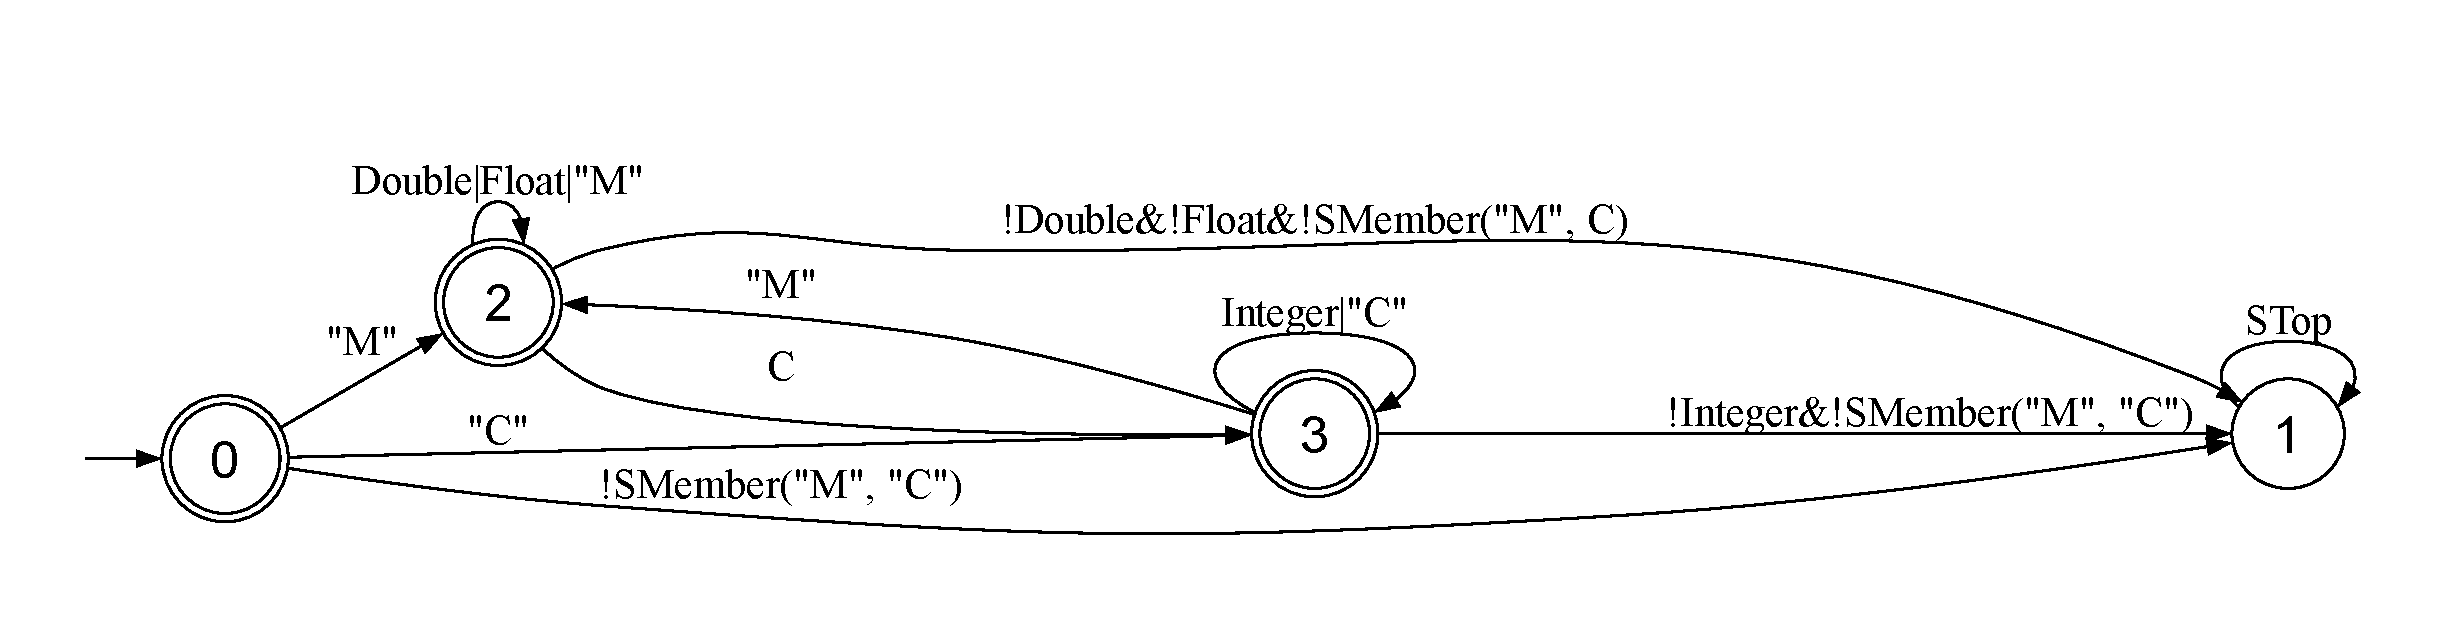
\includegraphics[width=0.9\textwidth]{example1.pdf}
\end{frame}


\begin{frame}{Example}{DFA, omitting sink state}
  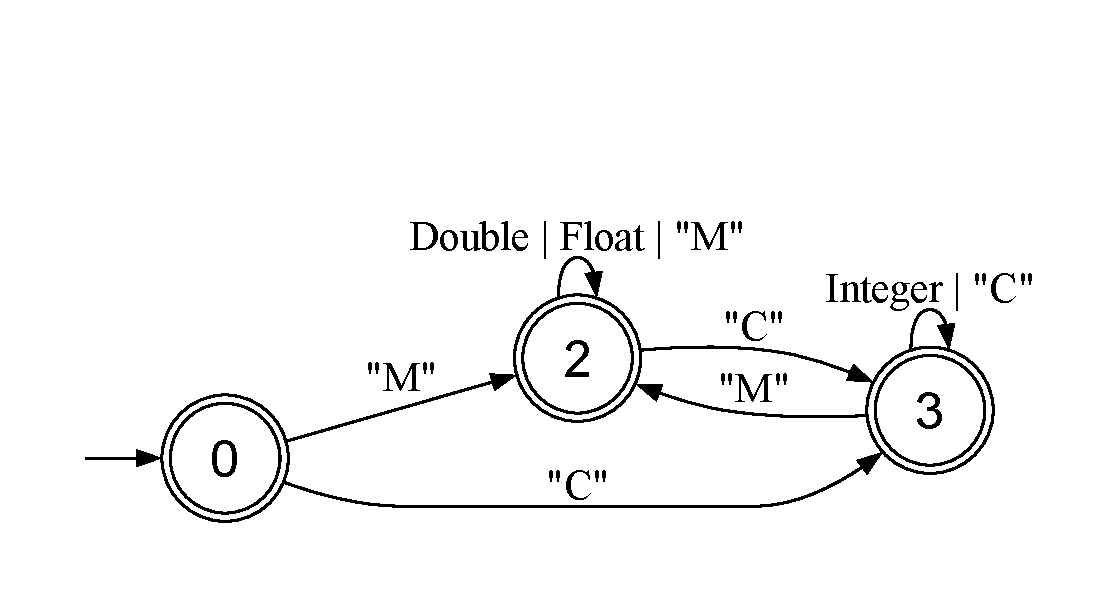
\includegraphics[width=0.9\textwidth]{example2.pdf}
\end{frame}

